\pgfdeclareplotmark{cross} {
\pgfpathmoveto{\pgfpoint{-0.3\pgfplotmarksize}{\pgfplotmarksize}}
\pgfpathlineto{\pgfpoint{+0.3\pgfplotmarksize}{\pgfplotmarksize}}
\pgfpathlineto{\pgfpoint{+0.3\pgfplotmarksize}{0.3\pgfplotmarksize}}
\pgfpathlineto{\pgfpoint{+1\pgfplotmarksize}{0.3\pgfplotmarksize}}
\pgfpathlineto{\pgfpoint{+1\pgfplotmarksize}{-0.3\pgfplotmarksize}}
\pgfpathlineto{\pgfpoint{+0.3\pgfplotmarksize}{-0.3\pgfplotmarksize}}
\pgfpathlineto{\pgfpoint{+0.3\pgfplotmarksize}{-1.\pgfplotmarksize}}
\pgfpathlineto{\pgfpoint{-0.3\pgfplotmarksize}{-1.\pgfplotmarksize}}
\pgfpathlineto{\pgfpoint{-0.3\pgfplotmarksize}{-0.3\pgfplotmarksize}}
\pgfpathlineto{\pgfpoint{-1.\pgfplotmarksize}{-0.3\pgfplotmarksize}}
\pgfpathlineto{\pgfpoint{-1.\pgfplotmarksize}{0.3\pgfplotmarksize}}
\pgfpathlineto{\pgfpoint{-0.3\pgfplotmarksize}{0.3\pgfplotmarksize}}
\pgfpathclose
\pgfusepathqstroke
}
\pgfdeclareplotmark{cross*} {
\pgfpathmoveto{\pgfpoint{-0.3\pgfplotmarksize}{\pgfplotmarksize}}
\pgfpathlineto{\pgfpoint{+0.3\pgfplotmarksize}{\pgfplotmarksize}}
\pgfpathlineto{\pgfpoint{+0.3\pgfplotmarksize}{0.3\pgfplotmarksize}}
\pgfpathlineto{\pgfpoint{+1\pgfplotmarksize}{0.3\pgfplotmarksize}}
\pgfpathlineto{\pgfpoint{+1\pgfplotmarksize}{-0.3\pgfplotmarksize}}
\pgfpathlineto{\pgfpoint{+0.3\pgfplotmarksize}{-0.3\pgfplotmarksize}}
\pgfpathlineto{\pgfpoint{+0.3\pgfplotmarksize}{-1.\pgfplotmarksize}}
\pgfpathlineto{\pgfpoint{-0.3\pgfplotmarksize}{-1.\pgfplotmarksize}}
\pgfpathlineto{\pgfpoint{-0.3\pgfplotmarksize}{-0.3\pgfplotmarksize}}
\pgfpathlineto{\pgfpoint{-1.\pgfplotmarksize}{-0.3\pgfplotmarksize}}
\pgfpathlineto{\pgfpoint{-1.\pgfplotmarksize}{0.3\pgfplotmarksize}}
\pgfpathlineto{\pgfpoint{-0.3\pgfplotmarksize}{0.3\pgfplotmarksize}}
\pgfpathclose
\pgfusepathqfillstroke
}
\pgfdeclareplotmark{newstar} {
\pgfpathmoveto{\pgfqpoint{0pt}{\pgfplotmarksize}}
\pgfpathlineto{\pgfqpointpolar{44}{0.5\pgfplotmarksize}}
\pgfpathlineto{\pgfqpointpolar{18}{\pgfplotmarksize}}
\pgfpathlineto{\pgfqpointpolar{-20}{0.5\pgfplotmarksize}}
\pgfpathlineto{\pgfqpointpolar{-54}{\pgfplotmarksize}}
\pgfpathlineto{\pgfqpointpolar{-90}{0.5\pgfplotmarksize}}
\pgfpathlineto{\pgfqpointpolar{234}{\pgfplotmarksize}}
\pgfpathlineto{\pgfqpointpolar{198}{0.5\pgfplotmarksize}}
\pgfpathlineto{\pgfqpointpolar{162}{\pgfplotmarksize}}
\pgfpathlineto{\pgfqpointpolar{134}{0.5\pgfplotmarksize}}
\pgfpathclose
\pgfusepathqstroke
}
\pgfdeclareplotmark{newstar*} {
\pgfpathmoveto{\pgfqpoint{0pt}{\pgfplotmarksize}}
\pgfpathlineto{\pgfqpointpolar{44}{0.5\pgfplotmarksize}}
\pgfpathlineto{\pgfqpointpolar{18}{\pgfplotmarksize}}
\pgfpathlineto{\pgfqpointpolar{-20}{0.5\pgfplotmarksize}}
\pgfpathlineto{\pgfqpointpolar{-54}{\pgfplotmarksize}}
\pgfpathlineto{\pgfqpointpolar{-90}{0.5\pgfplotmarksize}}
\pgfpathlineto{\pgfqpointpolar{234}{\pgfplotmarksize}}
\pgfpathlineto{\pgfqpointpolar{198}{0.5\pgfplotmarksize}}
\pgfpathlineto{\pgfqpointpolar{162}{\pgfplotmarksize}}
\pgfpathlineto{\pgfqpointpolar{134}{0.5\pgfplotmarksize}}
\pgfpathclose
\pgfusepathqfillstroke
}
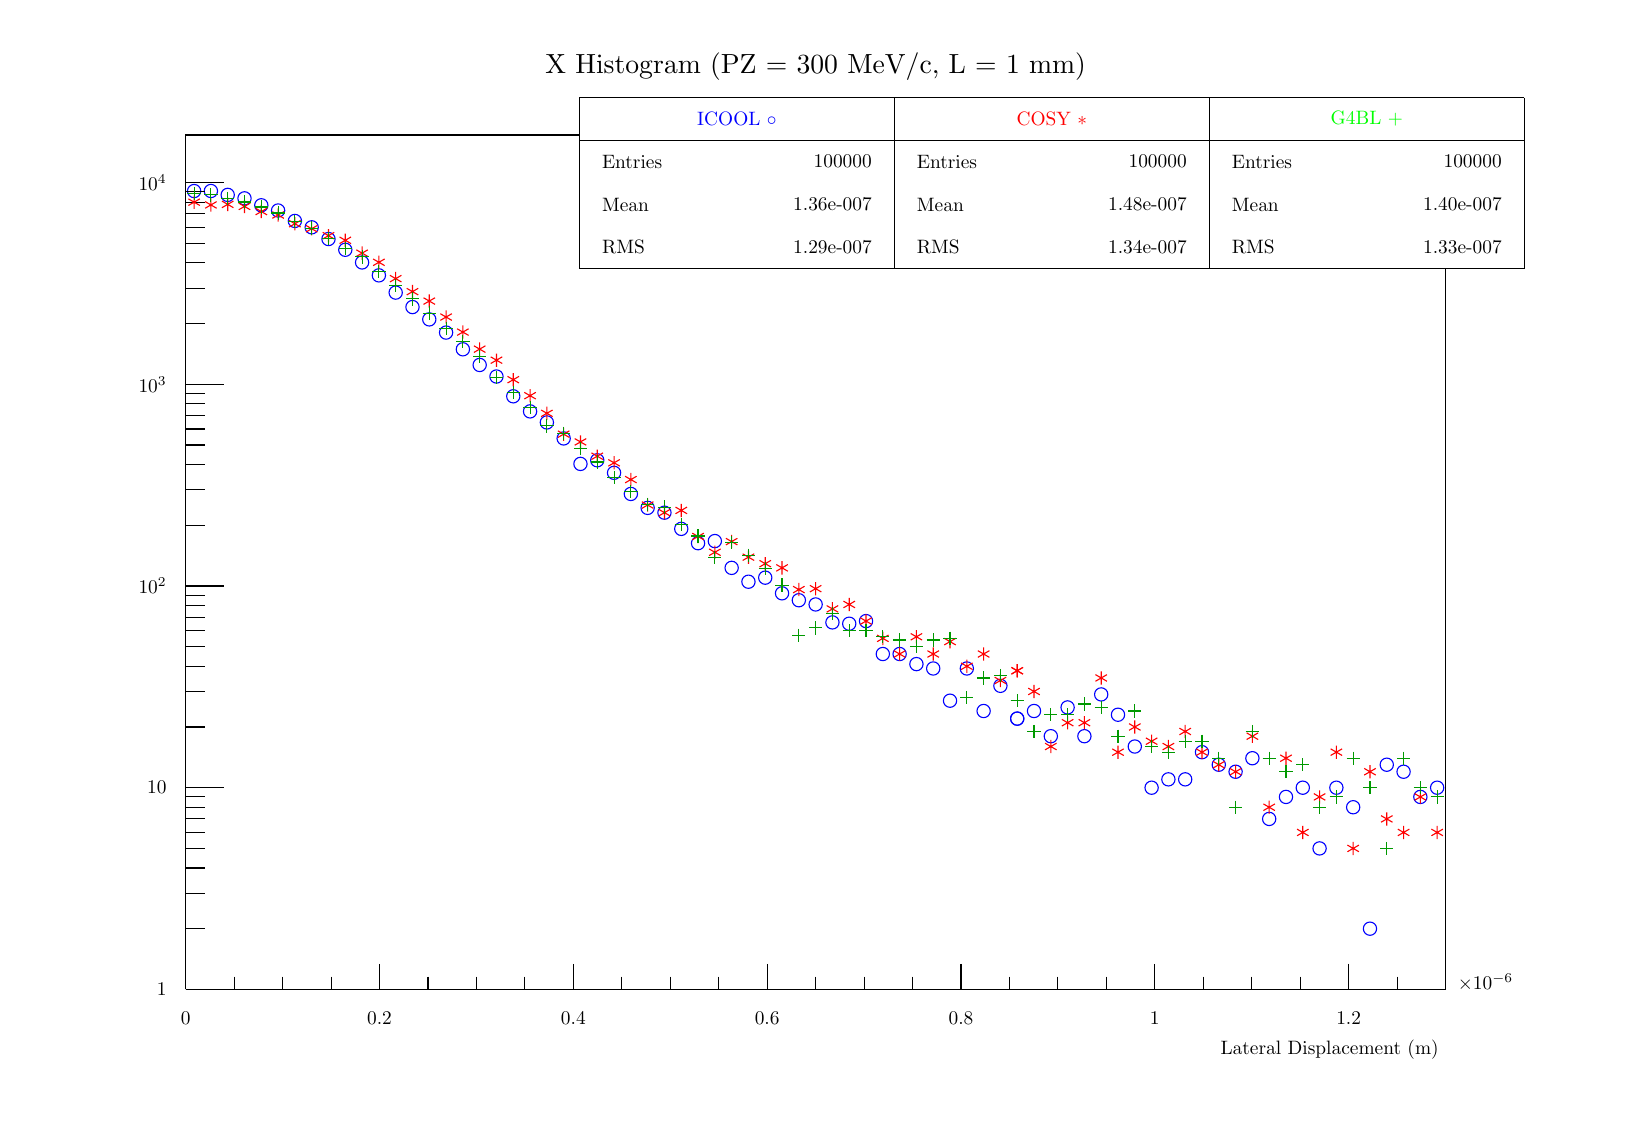
\begin{tikzpicture}
\definecolor{c}{rgb}{1,1,1};
\draw [color=c, fill=c] (0,0) rectangle (20,13.5632);
\draw [color=c, fill=c] (2,1.35632) rectangle (18,12.2069);
\definecolor{c}{rgb}{0,0,0};
\draw [c] (2,1.35632) -- (2,12.2069) -- (18,12.2069) -- (18,1.35632) -- (2,1.35632);
\definecolor{c}{rgb}{1,1,1};
\draw [color=c, fill=c] (2,1.35632) rectangle (18,12.2069);
\definecolor{c}{rgb}{0,0,0};
\draw [c] (2,1.35632) -- (2,12.2069) -- (18,12.2069) -- (18,1.35632) -- (2,1.35632);
\definecolor{c}{rgb}{0,0,1};
\foreach \P in
 {(2.10667,11.4951),(2.32,11.4959),(2.53333,11.4464),(2.74667,11.4024),(2.96,11.3145),(3.17333,11.2482),(3.38667,11.1154),(3.6,11.0343),(3.81333,10.886),(4.02667,10.7495),(4.24,10.5885),(4.45333,10.4245),(4.66667,10.2057),(4.88,10.0219),(5.09333,9.86
533),(5.30667,9.69799),(5.52,9.48538),(5.73333,9.28657),(5.94667,9.13993),(6.16,8.88864),(6.37333,8.69698),(6.58667,8.55663),(6.8,8.35345),(7.01333,8.02997),(7.22667,8.07594),(7.44,7.91674),(7.65333,7.64845),(7.86667,7.47177),(8.08,7.41086),(8.29333,
7.20514),(8.50667,7.02298),(8.72,7.04995),(8.93333,6.70974),(9.14667,6.53372),(9.36,6.58547),(9.57333,6.38669),(9.78667,6.29865),(10,6.24502),(10.2133,6.0172),(10.4267,6.00021),(10.64,6.03393),(10.8533,5.61558),(11.0667,5.61558),(11.28,5.48757),(11.4
933,5.43193),(11.7067,5.02285),(11.92,5.43193),(12.1333,4.89182),(12.3467,5.21186),(12.56,4.79502)}{\draw[mark options={color=c,fill=c},mark size=2.402402pt,mark=o] plot coordinates {\P};}
\foreach \P in
 {(12.56,4.79502),(12.7733,4.89182),(12.9867,4.57178),(13.2,4.93723),(13.4133,4.57178),(13.6267,5.10234),(13.84,4.84447),(14.0533,4.44075),(14.2667,3.91788),(14.48,4.02391),(14.6933,4.02391),(14.9067,4.36895),(15.12,4.20976),(15.3333,4.12071),(15.546
7,4.2922),(15.76,3.52109),(15.9733,3.80067),(16.1867,3.91788),(16.4,3.14678),(16.6133,3.91788),(16.8267,3.66964),(17.04,2.12743),(17.2533,4.20976),(17.4667,4.12071),(17.68,3.80067),(17.8933,3.91788)}{\draw[mark options={color=c,fill=c},mark
 size=2.402402pt,mark=o] plot coordinates {\P};}
\definecolor{c}{rgb}{1,1,1};
\draw [color=c, fill=c] (7,10.5115) rectangle (11,12.6816);
\definecolor{c}{rgb}{0,0,0};
\draw [c] (7,10.5115) -- (11,10.5115);
\draw [c] (11,10.5115) -- (11,12.6816);
\draw [c] (11,12.6816) -- (7,12.6816);
\draw [c] (7,12.6816) -- (7,10.5115);
\draw[color=blue](9,12.4103) node[scale=0.7, rotate=0]{ICOOL $\circ$};
\draw [c] (7,12.1391) -- (11,12.1391);
\draw [anchor= west] (7.2,11.8678) node[scale=0.7, rotate=0]{Entries };
\draw [anchor= east] (10.8,11.8678) node[scale=0.7, rotate=0]{ 100000};
\draw [anchor= west] (7.2,11.3253) node[scale=0.7, rotate=0]{Mean  };
\draw [anchor= east] (10.8,11.3253) node[scale=0.7, rotate=0]{ 1.36e-007};
\draw [anchor= west] (7.2,10.7828) node[scale=0.7, rotate=0]{RMS   };
\draw [anchor= east] (10.8,10.7828) node[scale=0.7, rotate=0]{ 1.29e-007};
\draw [c] (2,1.35632) -- (18,1.35632);
\draw [anchor= east] (18,0.596782) node[scale=0.7, rotate=0]{Lateral Displacement (m)};
\draw [c] (2,1.68184) -- (2,1.35632);
\draw [c] (2.61538,1.51908) -- (2.61538,1.35632);
\draw [c] (3.23077,1.51908) -- (3.23077,1.35632);
\draw [c] (3.84615,1.51908) -- (3.84615,1.35632);
\draw [c] (4.46154,1.68184) -- (4.46154,1.35632);
\draw [c] (5.07692,1.51908) -- (5.07692,1.35632);
\draw [c] (5.69231,1.51908) -- (5.69231,1.35632);
\draw [c] (6.30769,1.51908) -- (6.30769,1.35632);
\draw [c] (6.92308,1.68184) -- (6.92308,1.35632);
\draw [c] (7.53846,1.51908) -- (7.53846,1.35632);
\draw [c] (8.15385,1.51908) -- (8.15385,1.35632);
\draw [c] (8.76923,1.51908) -- (8.76923,1.35632);
\draw [c] (9.38461,1.68184) -- (9.38461,1.35632);
\draw [c] (10,1.51908) -- (10,1.35632);
\draw [c] (10.6154,1.51908) -- (10.6154,1.35632);
\draw [c] (11.2308,1.51908) -- (11.2308,1.35632);
\draw [c] (11.8462,1.68184) -- (11.8462,1.35632);
\draw [c] (12.4615,1.51908) -- (12.4615,1.35632);
\draw [c] (13.0769,1.51908) -- (13.0769,1.35632);
\draw [c] (13.6923,1.51908) -- (13.6923,1.35632);
\draw [c] (14.3077,1.68184) -- (14.3077,1.35632);
\draw [c] (14.9231,1.51908) -- (14.9231,1.35632);
\draw [c] (15.5385,1.51908) -- (15.5385,1.35632);
\draw [c] (16.1538,1.51908) -- (16.1538,1.35632);
\draw [c] (16.7692,1.68184) -- (16.7692,1.35632);
\draw [c] (16.7692,1.68184) -- (16.7692,1.35632);
\draw [c] (17.3846,1.51908) -- (17.3846,1.35632);
\draw [c] (18,1.51908) -- (18,1.35632);
\draw [anchor=base] (2,0.908736) node[scale=0.7, rotate=0]{0};
\draw [anchor=base] (4.46154,0.908736) node[scale=0.7, rotate=0]{0.2};
\draw [anchor=base] (6.92308,0.908736) node[scale=0.7, rotate=0]{0.4};
\draw [anchor=base] (9.38461,0.908736) node[scale=0.7, rotate=0]{0.6};
\draw [anchor=base] (11.8462,0.908736) node[scale=0.7, rotate=0]{0.8};
\draw [anchor=base] (14.3077,0.908736) node[scale=0.7, rotate=0]{1};
\draw [anchor=base] (16.7692,0.908736) node[scale=0.7, rotate=0]{1.2};
\draw [anchor=base west] (18.07,1.35632) node[scale=0.7, rotate=0]{$\times10^{-6}$};
\draw [c] (2,1.35632) -- (2,12.2069);
\draw [c] (2.48,1.35632) -- (2,1.35632);
\draw [anchor= east] (1.844,1.35632) node[scale=0.7, rotate=0]{1};
\draw [c] (2.24,2.12743) -- (2,2.12743);
\draw [c] (2.24,2.5785) -- (2,2.5785);
\draw [c] (2.24,2.89854) -- (2,2.89854);
\draw [c] (2.24,3.14678) -- (2,3.14678);
\draw [c] (2.24,3.34961) -- (2,3.34961);
\draw [c] (2.24,3.52109) -- (2,3.52109);
\draw [c] (2.24,3.66964) -- (2,3.66964);
\draw [c] (2.24,3.80067) -- (2,3.80067);
\draw [c] (2.48,3.91789) -- (2,3.91789);
\draw [anchor= east] (1.844,3.91789) node[scale=0.7, rotate=0]{10};
\draw [c] (2.24,4.68899) -- (2,4.68899);
\draw [c] (2.24,5.14006) -- (2,5.14006);
\draw [c] (2.24,5.4601) -- (2,5.4601);
\draw [c] (2.24,5.70834) -- (2,5.70834);
\draw [c] (2.24,5.91117) -- (2,5.91117);
\draw [c] (2.24,6.08266) -- (2,6.08266);
\draw [c] (2.24,6.23121) -- (2,6.23121);
\draw [c] (2.24,6.36224) -- (2,6.36224);
\draw [c] (2.48,6.47945) -- (2,6.47945);
\draw [anchor= east] (1.844,6.47945) node[scale=0.7, rotate=0]{$10^{2}$};
\draw [c] (2.24,7.25055) -- (2,7.25055);
\draw [c] (2.24,7.70162) -- (2,7.70162);
\draw [c] (2.24,8.02166) -- (2,8.02166);
\draw [c] (2.24,8.2699) -- (2,8.2699);
\draw [c] (2.24,8.47273) -- (2,8.47273);
\draw [c] (2.24,8.64422) -- (2,8.64422);
\draw [c] (2.24,8.79277) -- (2,8.79277);
\draw [c] (2.24,8.9238) -- (2,8.9238);
\draw [c] (2.48,9.04101) -- (2,9.04101);
\draw [anchor= east] (1.844,9.04101) node[scale=0.7, rotate=0]{$10^{3}$};
\draw [c] (2.24,9.81211) -- (2,9.81211);
\draw [c] (2.24,10.2632) -- (2,10.2632);
\draw [c] (2.24,10.5832) -- (2,10.5832);
\draw [c] (2.24,10.8315) -- (2,10.8315);
\draw [c] (2.24,11.0343) -- (2,11.0343);
\draw [c] (2.24,11.2058) -- (2,11.2058);
\draw [c] (2.24,11.3543) -- (2,11.3543);
\draw [c] (2.24,11.4854) -- (2,11.4854);
\draw [c] (2.48,11.6026) -- (2,11.6026);
\draw [anchor= east] (1.844,11.6026) node[scale=0.7, rotate=0]{$10^{4}$};
\definecolor{c}{rgb}{1,1,1};
\draw [color=c, fill=c] (7,10.5115) rectangle (11,12.6816);
\definecolor{c}{rgb}{0,0,0};
\draw [c] (7,10.5115) -- (11,10.5115);
\draw [c] (11,10.5115) -- (11,12.6816);
\draw [c] (11,12.6816) -- (7,12.6816);
\draw [c] (7,12.6816) -- (7,10.5115);
\draw[color=blue](9,12.4103) node[scale=0.7, rotate=0]{ICOOL $\circ$};
\draw [c] (7,12.1391) -- (11,12.1391);
\draw [anchor= west] (7.2,11.8678) node[scale=0.7, rotate=0]{Entries };
\draw [anchor= east] (10.8,11.8678) node[scale=0.7, rotate=0]{ 100000};
\draw [anchor= west] (7.2,11.3253) node[scale=0.7, rotate=0]{Mean  };
\draw [anchor= east] (10.8,11.3253) node[scale=0.7, rotate=0]{ 1.36e-007};
\draw [anchor= west] (7.2,10.7828) node[scale=0.7, rotate=0]{RMS   };
\draw [anchor= east] (10.8,10.7828) node[scale=0.7, rotate=0]{ 1.29e-007};
\draw (10,13.0816) node[scale=1, rotate=0]{X Histogram (PZ = 300 MeV/c, L = 1 mm)};
\definecolor{c}{rgb}{1,0,0};
\foreach \P in
 {(2.10667,11.354),(2.32,11.3189),(2.53333,11.326),(2.74667,11.2998),(2.96,11.2348),(3.17333,11.1911),(3.38667,11.0802),(3.6,11.0167),(3.81333,10.9286),(4.02667,10.8699),(4.24,10.7068),(4.45333,10.5904),(4.66667,10.3829),(4.88,10.2178),(5.09333,10.09
8),(5.30667,9.89515),(5.52,9.70413),(5.73333,9.48762),(5.94667,9.34733),(6.16,9.09951),(6.37333,8.89626),(6.58667,8.67246),(6.8,8.40783),(7.01333,8.30925),(7.22667,8.12769),(7.44,8.04369),(7.65333,7.831),(7.86667,7.50766),(8.08,7.41086),(8.29333,7.43
939),(8.50667,7.10834),(8.72,6.90804),(8.93333,7.04327),(9.14667,6.84579),(9.36,6.76273),(9.57333,6.70974),(9.78667,6.43403),(10,6.44556),(10.2133,6.18868),(10.4267,6.24502),(10.64,6.03393),(10.8533,5.81437),(11.0667,5.61558),(11.28,5.83441),(11.4933
,5.61558),(11.7067,5.77316),(11.92,5.4601),(12.1333,5.61558),(12.3467,5.2793),(12.56,5.40304)}{\draw[mark options={color=c,fill=c},mark size=2.402402pt,mark=asterisk] plot coordinates {\P};}
\foreach \P in
 {(12.56,5.40304),(12.7733,5.14006),(12.9867,4.44075),(13.2,4.74327),(13.4133,4.74327),(13.6267,5.31155),(13.84,4.36895),(14.0533,4.68899),(14.2667,4.50819),(14.48,4.44075),(14.6933,4.63193),(14.9067,4.36895),(15.12,4.20976),(15.3333,4.12071),(15.546
7,4.57178),(15.76,3.66964),(15.9733,4.2922),(16.1867,3.3496),(16.4,3.80067),(16.6133,4.36895),(16.8267,3.14678),(17.04,4.12071),(17.2533,3.52109),(17.4667,3.3496),(17.68,3.80067),(17.8933,3.3496)}{\draw[mark options={color=c,fill=c},mark
 size=2.402402pt,mark=asterisk] plot coordinates {\P};}
\definecolor{c}{rgb}{1,1,1};
\draw [color=c, fill=c] (11,10.5115) rectangle (15,12.6816);
\definecolor{c}{rgb}{0,0,0};
\draw [c] (11,10.5115) -- (15,10.5115);
\draw [c] (15,10.5115) -- (15,12.6816);
\draw [c] (15,12.6816) -- (11,12.6816);
\draw [c] (11,12.6816) -- (11,10.5115);
\draw [color=red](13,12.4103) node[scale=0.7, rotate=0]{COSY $*$};
\draw [c] (11,12.1391) -- (15,12.1391);
\draw [anchor= west] (11.2,11.8678) node[scale=0.7, rotate=0]{Entries };
\draw [anchor= east] (14.8,11.8678) node[scale=0.7, rotate=0]{ 100000};
\draw [anchor= west] (11.2,11.3253) node[scale=0.7, rotate=0]{Mean  };
\draw [anchor= east] (14.8,11.3253) node[scale=0.7, rotate=0]{ 1.48e-007};
\draw [anchor= west] (11.2,10.7828) node[scale=0.7, rotate=0]{RMS   };
\draw [anchor= east] (14.8,10.7828) node[scale=0.7, rotate=0]{ 1.34e-007};
\definecolor{c}{rgb}{1,1,1};
\draw [color=c, fill=c] (11,10.5115) rectangle (15,12.6816);
\definecolor{c}{rgb}{0,0,0};
\draw [c] (11,10.5115) -- (15,10.5115);
\draw [c] (15,10.5115) -- (15,12.6816);
\draw [c] (15,12.6816) -- (11,12.6816);
\draw [c] (11,12.6816) -- (11,10.5115);
\draw [color=red](13,12.4103) node[scale=0.7, rotate=0]{COSY $*$};
\draw [c] (11,12.1391) -- (15,12.1391);
\draw [anchor= west] (11.2,11.8678) node[scale=0.7, rotate=0]{Entries };
\draw [anchor= east] (14.8,11.8678) node[scale=0.7, rotate=0]{ 100000};
\draw [anchor= west] (11.2,11.3253) node[scale=0.7, rotate=0]{Mean  };
\draw [anchor= east] (14.8,11.3253) node[scale=0.7, rotate=0]{ 1.48e-007};
\draw [anchor= west] (11.2,10.7828) node[scale=0.7, rotate=0]{RMS   };
\draw [anchor= east] (14.8,10.7828) node[scale=0.7, rotate=0]{ 1.34e-007};
\definecolor{c}{rgb}{0,0.6,0};
\foreach \P in
 {(2.10667,11.4624),(2.32,11.4462),(2.53333,11.4002),(2.74667,11.3567),(2.96,11.2933),(3.17333,11.2162),(3.38667,11.1089),(3.6,11.025),(3.81333,10.8965),(4.02667,10.7617),(4.24,10.659),(4.45333,10.4725),(4.66667,10.2935),(4.88,10.1252),(5.09333,9.945
12),(5.30667,9.74564),(5.52,9.58249),(5.73333,9.39609),(5.94667,9.12353),(6.16,8.94097),(6.37333,8.743),(6.58667,8.51279),(6.8,8.41761),(7.01333,8.22911),(7.22667,8.05454),(7.44,7.85387),(7.65333,7.68292),(7.86667,7.51645),(8.08,7.48085),(8.29333,7.2
6162),(8.50667,7.11464),(8.72,6.83775),(8.93333,7.02978),(9.14667,6.86954),(9.36,6.70066),(9.57333,6.49051),(9.78667,5.8541),(10,5.94764),(10.2133,6.12934),(10.4267,5.91117),(10.64,5.91117),(10.8533,5.83441),(11.0667,5.79396),(11.28,5.70834),(11.4933
,5.79396),(11.7067,5.81437),(11.92,5.06331),(12.1333,5.31155),(12.3467,5.34289),(12.56,5.02285)}{\draw[mark options={color=c,fill=c},mark size=2.402402pt,mark=+] plot coordinates {\P};}
\foreach \P in
 {(12.56,5.02285),(12.7733,4.63193),(12.9867,4.84447),(13.2,4.84447),(13.4133,4.98086),(13.6267,4.93723),(13.84,4.57178),(14.0533,4.89182),(14.2667,4.44075),(14.48,4.36895),(14.6933,4.50819),(14.9067,4.50819),(15.12,4.2922),(15.3333,3.66964),(15.5467
,4.63193),(15.76,4.2922),(15.9733,4.12071),(16.1867,4.20976),(16.4,3.66964),(16.6133,3.80067),(16.8267,4.2922),(17.04,3.91788),(17.2533,3.14678),(17.4667,4.2922),(17.68,3.91788),(17.8933,3.80067)}{\draw[mark options={color=c,fill=c},mark
 size=2.402402pt,mark=+] plot coordinates {\P};}
\definecolor{c}{rgb}{1,1,1};
\draw [color=c, fill=c] (15,10.5115) rectangle (19,12.6816);
\definecolor{c}{rgb}{0,0,0};
\draw [c] (15,10.5115) -- (19,10.5115);
\draw [c] (19,10.5115) -- (19,12.6816);
\draw [c] (19,12.6816) -- (15,12.6816);
\draw [c] (15,12.6816) -- (15,10.5115);
\draw [color=green](17,12.4103) node[scale=0.7, rotate=0]{G4BL $+$};
\draw [c] (15,12.1391) -- (19,12.1391);
\draw [anchor= west] (15.2,11.8678) node[scale=0.7, rotate=0]{Entries };
\draw [anchor= east] (18.8,11.8678) node[scale=0.7, rotate=0]{ 100000};
\draw [anchor= west] (15.2,11.3253) node[scale=0.7, rotate=0]{Mean  };
\draw [anchor= east] (18.8,11.3253) node[scale=0.7, rotate=0]{ 1.40e-007};
\draw [anchor= west] (15.2,10.7828) node[scale=0.7, rotate=0]{RMS   };
\draw [anchor= east] (18.8,10.7828) node[scale=0.7, rotate=0]{ 1.33e-007};
\definecolor{c}{rgb}{1,1,1};
\draw [color=c, fill=c] (15,10.5115) rectangle (19,12.6816);
\definecolor{c}{rgb}{0,0,0};
\draw [c] (15,10.5115) -- (19,10.5115);
\draw [c] (19,10.5115) -- (19,12.6816);
\draw [c] (19,12.6816) -- (15,12.6816);
\draw [c] (15,12.6816) -- (15,10.5115);
\draw [color=green](17,12.4103) node[scale=0.7, rotate=0]{G4BL $+$};
\draw [c] (15,12.1391) -- (19,12.1391);
\draw [anchor= west] (15.2,11.8678) node[scale=0.7, rotate=0]{Entries };
\draw [anchor= east] (18.8,11.8678) node[scale=0.7, rotate=0]{ 100000};
\draw [anchor= west] (15.2,11.3253) node[scale=0.7, rotate=0]{Mean  };
\draw [anchor= east] (18.8,11.3253) node[scale=0.7, rotate=0]{ 1.40e-007};
\draw [anchor= west] (15.2,10.7828) node[scale=0.7, rotate=0]{RMS   };
\draw [anchor= east] (18.8,10.7828) node[scale=0.7, rotate=0]{ 1.33e-007};
\end{tikzpicture}
